\part{Data Analysis and Dislaying}
\section{Analysis of the data}
Total implementation link for data analyzer : \\
\url{https://github.com/Sprea22/Data_Analyzer_Python}

During this part the main purpose is to analyse the whole dataset in order to find some kind of useful informations later on. \\
The Python system implemented in this section is mainly used for a generic analysis of the data from different point of views.\\
The output of this phase will basically be for each single data input:
\begin{itemize}
\item Total graphic of the input data from 2005 to 2016.
\item Graphic of the input data for each single year from 2005 to 2016.
\item Correlation matrix between different months of the same input.
\item Correlation matrix between different years of the same input.
\end{itemize}

And then it also provides:
\begin{itemize}
\item General correlation matrix between all the different inputs.
\item Graphic of the normalized angular coefficients of all the inputs.
\end{itemize}

It's important to remind that this phase can be implemented in different ways and with different programming language, in this case has been choose Python, so be sure to have installed all the necessary for compile and execute Python code on your platform.\\
Current development environment:\\
Python version: 2.7.12\\
Linux kernel version number: Linux Asus 4.4.0-71-generic SMP\\

During this experiment has been implemented a system that could be divided in two subsystems, that are:
\begin{itemize}
\item Single Input Analyzer (SIA): Used for analyze a single data input.
\item Multiple Inputs Analyzer (MIA): Used for analyze multiple data inputs.
\end{itemize}
\newpage


\newpage
\subsection{Single Input Analyzer}
\begin{itemize}
\item SIA imported libraries.
\item SIA part I: Generate and display a graphic about current input with total data from 2005 to 2016.
\item SIA part II: Generate and display a graphic about current input for each year from 2005 to 2016.
\item SIA part III: Generate and display a graphic that contains the correlation matrix between each single year from 2005 to 2016 of the current input.
\item SIA part IV: Generate and display a graphic that contains the correlation matrix between each single months of the year of the current input.
\item SIA part V: Generate and display a single overview image for the current input.
\end{itemize}

\subsubsection{SIA: Requirements for reusability}
The system that is going to be implemented in this phase of the work could be used for other data inputs as well, but there are of course some kind of requiriments about the dataset that are necessary for let it works in a proper way.\\
The aalysis system need in input a dataset structure that:
\begin{itemize}
\item Data from January 2005 to December 2016
\item One single value for each month
\end{itemize}
It means that the dataset must contains 144 values for each single input.
\newpage

\subsubsection{SIA section I: Total graphic for all the years}
\textbf{Goal:}\\
Generate and display the total graphic about current input from 2005 to 2016.

\textbf{Requirements:}\\
- Data content: 144 values, 1 value for each month from 2005 to 2016

\textbf{Implementation:}\\
It's possible to check out the full ccommented code in the appendice: \ref{SIA_section_I}

\textbf{Results:} \\
With this first part of the code has been reached the first goal of to displaying and save the basic graphic about the current input from 2005 to 2016, with also the trendline displayed, that looks like this example:

\begin{figure}[H]
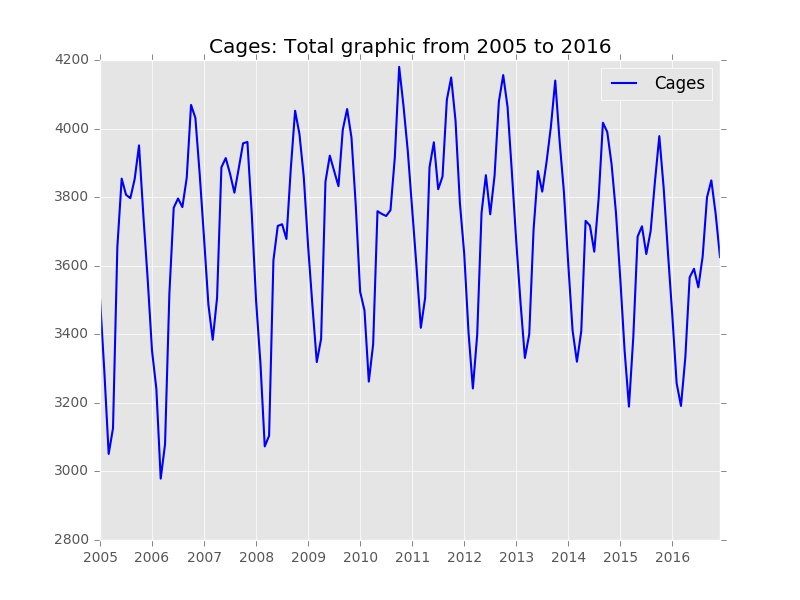
\includegraphics[width=1\textwidth]{Files/Cages_Total.jpg}
\caption{Total graphic about current input with total data from 2005 to 2016.}
\end{figure}



\newpage
\subsubsection{SIA section II: Single graphics for each year}

\textbf{Goal:}\\
Generate and display graphics about current input for each year from 2005 to 2016

\textbf{Requirements:}\\
- Data content: 144 values, 1 value for each month from 2005 to 2016

\textbf{Results:} \\
With this second part of the code has been reached the goal of displaying and save the graphics about the current input for each single year from 2005 to 2016, that looks like this example:

\begin{figure}[H]
	\centering
    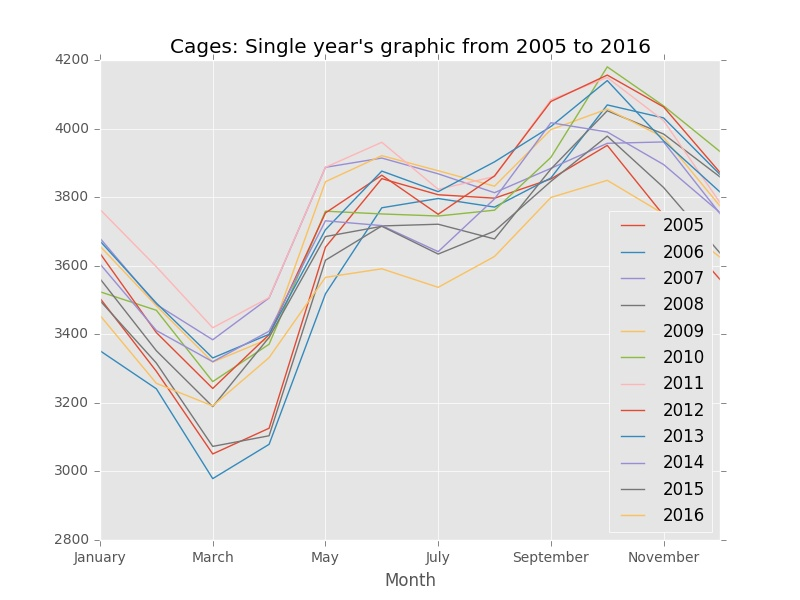
\includegraphics[width=1\textwidth]{Files/Cages_Years.jpg}
    \caption{Graphics for each single year of the input data from 2005 to 2016}
\end{figure}




\newpage
\subsubsection{SIA section III: Correlation matrix between years}

\textbf{Goal:}\\
Calculate the correlation coefficients between each single year from 2005 to 2016 of the current input and then display it with a correlation matrix.

\textbf{Requirements:}\\
- Data content: 144 values, 1 value for each month from 2005 to 2016



\textbf{Results:} \\
With this third part of the code have been calculated the correlation coefficients between each single year from 2005 to 2016 for each single inputs, saved the values in a document and then also displayed and saved the correlation matrix about it, that looks like this example:

\begin{figure}[H]
	\centering
    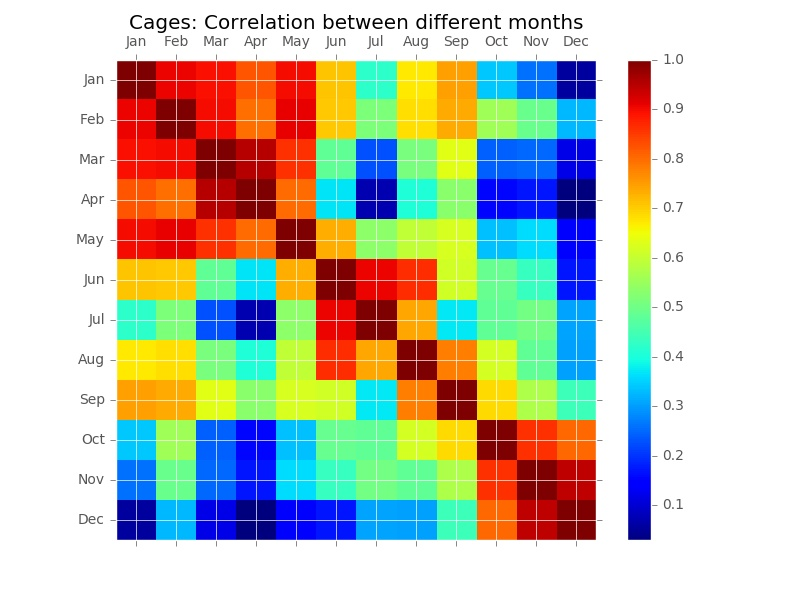
\includegraphics[width=1\textwidth]{Files/Cages_Months_Matrix.jpg}
    \caption{Correlation matrix between different months of the same input}
\end{figure}




\newpage
\subsubsection{SIA section IV: Correlation matrix between months}

\textbf{Goal:}\\
Calculate the correlation coefficients between each single month from 2005 to 2016 of the current input and then display it with a correlation matrix.

\textbf{Requirements:}\\
- Data content: 144 values, 1 value for each month from 2005 to 2016

\textbf{Results:} \\
With this part of the code have been calculated the correlation coefficients between each single month from 2005 to 2016 of all the inputs and saved it in a document. Then has been also displayed and saved the correlation matrix about it, that looks like this example:

\begin{figure}[H]
	\centering
    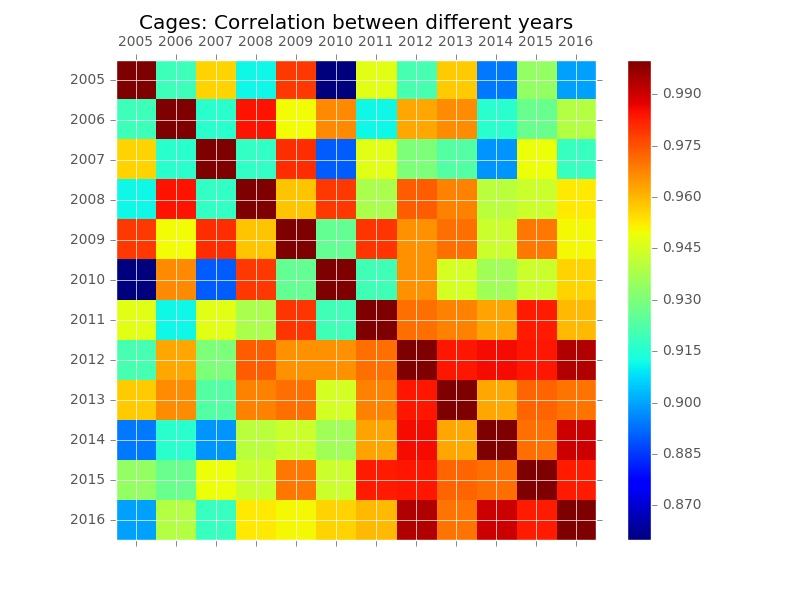
\includegraphics[width=1\textwidth]{Files/Cages_Years_Matrix.jpg}
    \caption{Correlation matrix between different years of the same input}
\end{figure}


\newpage
\subsubsection{SIA section V: Single overview}

\textbf{Goal:}\\
Generate and display a single overview image for the current input.

\textbf{Requirements:}\\
- All the images that contain graphic about current input.

\textbf{Results:}
\begin{figure}[H]
    \makebox[\textwidth][c]{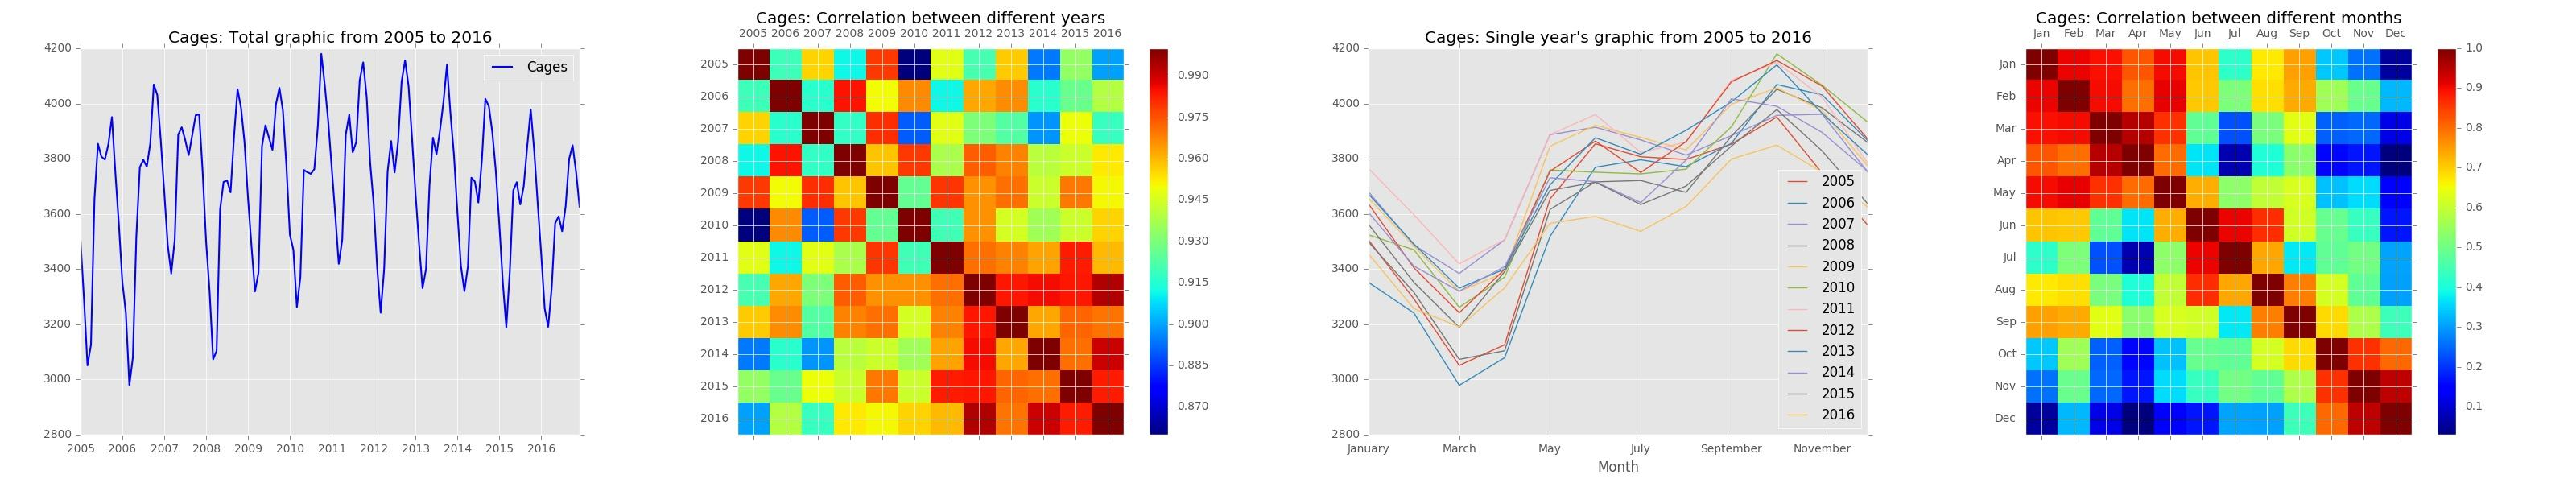
\includegraphics[width=1.2\textwidth]{Files/Cages_Overview.jpg}}
    \caption{Example of "Single Input Overview Image"}
\end{figure}

\newpage

\subsection{Multiple Inputs Analyzer}
\subsubsection{MIA: Requirements for reusability}
The system that is going to be implemented during this phase it's not reusable at all.
It means that has been implemneted just for analyze the current dataset composed by 8 different inputs about Aquaculture.

\subsubsection{MIA: Implementation}
\textbf{Goal:}\\
This analyzer is mainly used for show the correlation coefficent between the diffent inputs along the total period (from 2005 o 2016), that it will be important to have a general about which kind of relation there is between different inputs and how much strong it is.

\textbf{Requirements:}\\
- Input dataset: Total\_Dataset required, structure already reported here:
\hyperref[table: Total_Dataset]{Total Dataset}

\textbf{Results:} \\

\begin{figure}[H]
	\centering
    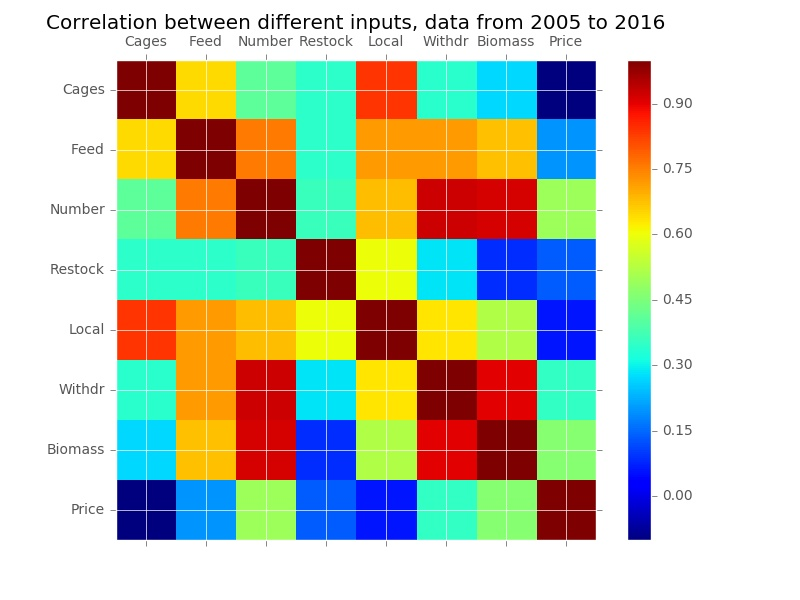
\includegraphics[width=0.75\textwidth]{Files/Total_Dataset_Years_Matrix.jpg}
    \caption{Correlation matrix between different inputs with data from 2005 to 2016.}
\end{figure}

\begin{figure}[H]
	\centering
    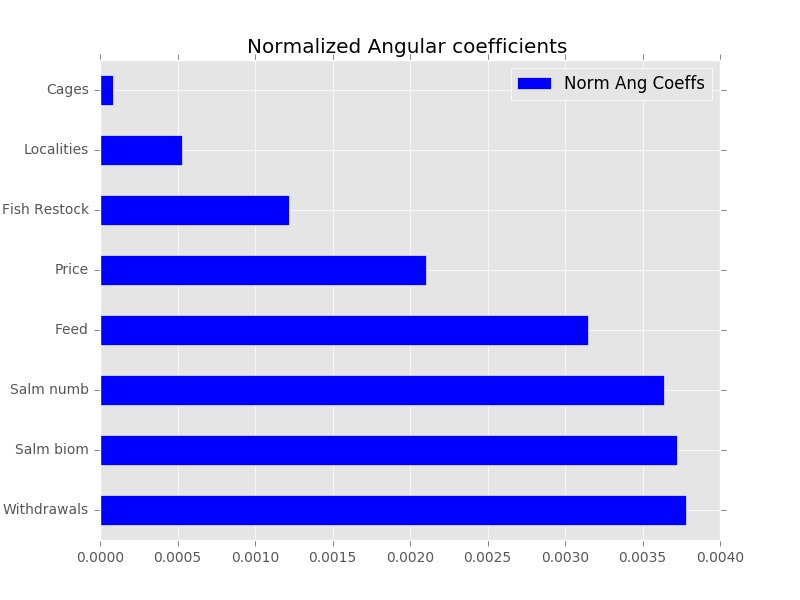
\includegraphics[width=0.75\textwidth]{Files/Norm_Ang_Coeffs.jpg}
    \caption{Normalized angular coefficients of each input's trendline.}
\end{figure}


\newpage
\section{Extract information from data}
